\documentclass[10pt,a4paper]{article}
\usepackage[utf8]{inputenc}
\usepackage{amsmath}
\usepackage{amsfonts}
\usepackage{amssymb}
\usepackage{graphicx}
\usepackage[varg]{txfonts}
\usepackage{geometry}
\geometry{
a4paper,
total={210mm,297mm},
left=20mm,
right=20mm,
top=20mm,
bottom=20mm,
hoffset=-10pt
}
\begin{document}
\title{Problems for Tutorial-04: \\Ordinary Differential equations}
\date{}
\maketitle
\begin{enumerate}
\item Find the solution of the differential equation at time $t = 10$ 
\begin{align*}
	\dot{x}_1 &= -x_1 + 3 x_2 + 2\\
	\dot{x}_2 &= -2 x_2 + 1
\end{align*}
Consider the initial condition be $(0.1,0.2)$ at $t = 0$. 
\item Plot the solution of the above differential $(x_1,x_2)$ for $t \in [0.2,10]$.
\end{enumerate}
{\bf Solution:}
\begin{figure}[ht!]
\raggedleft{
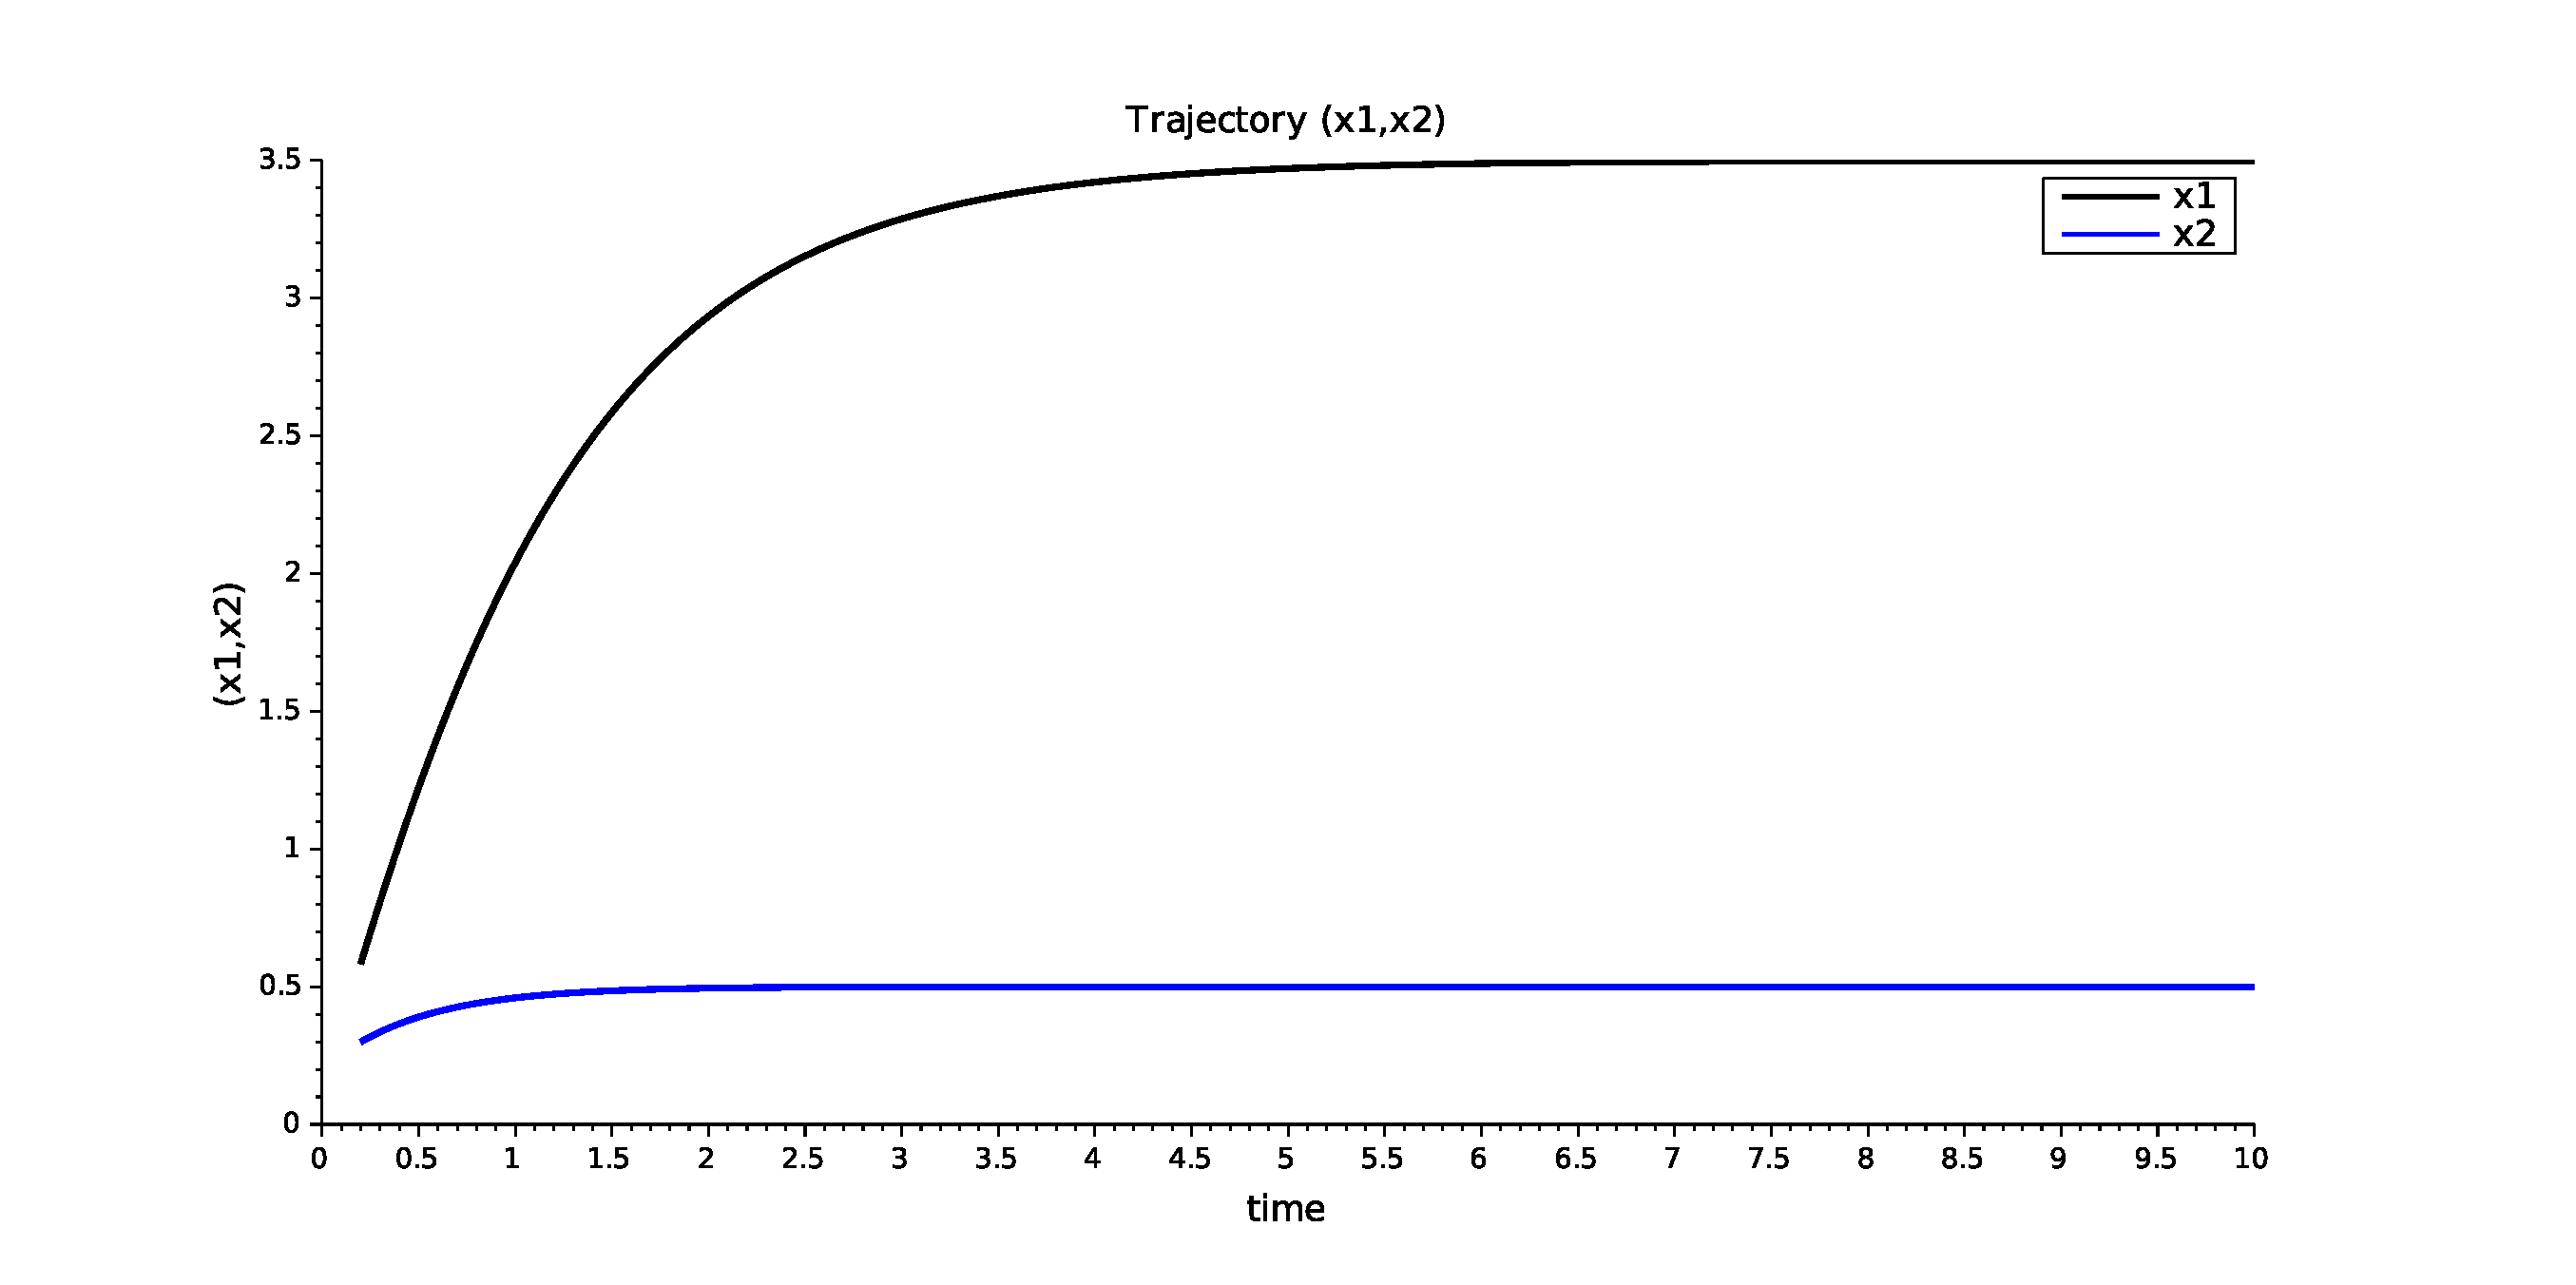
\includegraphics[scale=0.4]{SolPrblm04.pdf}}
\end{figure}
\end{document}
